%%%%%%%%%%%%%%%%%%%%%%%%%%%%%%%%%%%%%%%%%
% Daily Laboratory Book
% LaTeX Template
%
% This template has been downloaded from:
% http://www.latextemplates.com
%
% Original author:
% Frank Kuster (http://www.ctan.org/tex-archive/macros/latex/contrib/labbook/)
%
% Important note:
% This template requires the labbook.cls file to be in the same directory as the
% .tex file. The labbook.cls file provides the necessary structure to create the
% lab book.
%
% The \lipsum[#] commands throughout this template generate dummy text
% to fill the template out. These commands should all be removed when 
% writing lab book content.
%
% HOW TO USE THIS TEMPLATE 
% Each day in the lab consists of three main things:
%
% 1. LABDAY: The first thing to put is the \labday{} command with a date in 
% curly brackets, this will make a new page and put the date in big letters 
% at the top.
%
% 2. EXPERIMENT: Next you need to specify what experiment(s) you are 
% working on with an \experiment{} command with the experiment shorthand 
% in the curly brackets. The experiment shorthand is defined in the 
% 'DEFINITION OF EXPERIMENTS' section below, this means you can 
% say \experiment{pcr} and the actual text written to the PDF will be what 
% you set the 'pcr' experiment to be. If the experiment is a one off, you can 
% just write it in the bracket without creating a shorthand. Note: if you don't 
% want to have an experiment, just leave this out and it won't be printed.
%
% 3. CONTENT: Following the experiment is the content, i.e. what progress 
% you made on the experiment that day.
%
%%%%%%%%%%%%%%%%%%%%%%%%%%%%%%%%%%%%%%%%%

%----------------------------------------------------------------------------------------
%	PACKAGES AND OTHER DOCUMENT CONFIGURATIONS
%----------------------------------------------------------------------------------------

\documentclass[idxtotoc,hyperref,openany]{labbook} % 'openany' here removes the gap page between days, erase it to restore this gap; 'oneside' can also be added to remove the shift that odd pages have to the right for easier reading

\usepackage[ 
  backref=page,
  pdfpagelabels=true,
  plainpages=false,
  colorlinks=true,
  bookmarks=true,
  pdfview=FitB]{hyperref} % Required for the hyperlinks within the PDF
\usepackage{booktabs} % Required for the top and bottom rules in the table
\usepackage{float} % Required for specifying the exact location of a figure or table
\usepackage{graphicx} % Required for including images
\usepackage{lipsum} % Used for inserting dummy 'Lorem ipsum' text into the template
\usepackage{listings}
\usepackage{color}
\usepackage{mathtools}
\usepackage[spanish]{babel}
\definecolor{codegreen}{rgb}{0,0.6,0}
\definecolor{codegray}{rgb}{0.5,0.5,0.5}
\definecolor{codepurple}{rgb}{0.58,0,0.82}
\definecolor{backcolour}{rgb}{0.95,0.95,0.92}

\lstdefinestyle{mystyle}{
    backgroundcolor=\color{backcolour},   
    commentstyle=\color{codegreen},
    keywordstyle=\color{magenta},
    numberstyle=\tiny\color{codegray},
    stringstyle=\color{codepurple},
    basicstyle=\footnotesize,
    breakatwhitespace=false,         
    breaklines=true,                 
    captionpos=b,                    
    keepspaces=true,                 
    numbers=left,                    
    numbersep=5pt,                  
    showspaces=false,                
    showstringspaces=false,
    showtabs=false,                  
    tabsize=2
}

\lstset{style=mystyle}

\newcommand{\HRule}{\rule{\linewidth}{0.5mm}} % Command to make the lines in the title page
\setlength\parindent{0pt} % Removes all indentation from paragraphs

%----------------------------------------------------------------------------------------
%	DEFINITION OF EXPERIMENTS
%----------------------------------------------------------------------------------------

\newexperiment{example}{This is an example experiment}
\newexperiment{example2}{This is another example experiment}
\newexperiment{example3}{This is yet another example experiment}
\newexperiment{table}{This shows a sample table}
%\newexperiment{shorthand}{Description of the experiment}

%---------------------------------------------------------------------------------------

\begin{document}

%----------------------------------------------------------------------------------------
%	TITLE PAGE
%----------------------------------------------------------------------------------------

\frontmatter % Use Roman numerals for page numbers
\title{
\begin{center}
\HRule \\[0.4cm]
{\Huge \bfseries Bitácora de la tesis \\[0.5cm] \Large Pregrado de Física}\\[0.4cm] % Degree
\HRule \\[1.5cm]
\end{center}
}
\author{\Huge Santiago Peña Martínez \\ \\ \LARGE spenam@unal.edu.co \\[2cm]} % Your name and email address
\date{Inicio 7 Febrero 2019} % Beginning date
\maketitle

\tableofcontents

\mainmatter % Use Arabic numerals for page numbers

%----------------------------------------------------------------------------------------
%	LAB BOOK CONTENTS
%----------------------------------------------------------------------------------------

% Blank template to use for new days:

%\labday{Day, Date Month Year}

%\experiment{}

%Text

%-----------------------------------------

%\experiment{}

%Text

%----------------------------------------------------------------------------------------

\labday{Jueves, 7 Febrero 2019}

\experiment{Inicio de la carrera contra reloj}

Hoy en la tarde estuve hablando con Óscar, le conté de mis ideas sobre terminar temprano la tésis y acabar la carrera pronto con el fin de irme a Japón. Él se mostró muy entusiasmado con mi idea, me dio consejos para posiblemente llevar a cabo esta tarea (incluyendo el de hacer una bitácora). Esta bitácora va a ser un poco narrativa almismo tiempo de técnica, creo que acá podría expresar mis pensamientos y quizá leerlos en un futuro cuando no tenga nada que hacer, recordar lo que pensaba cuando tenía 20 años y comparar con lo que esté haciendo ahora.\par

Como soy distraído, estaba estudiando para el parcial del martes de Ondas y recordé que tenía que hacer la bitácora, decidí buscar un template en internet y empezarla ya que de lo contrario puede que nunca la empiece.\par
Hoy no tengo pensado avanzar en cuanto al proyecto debido al parcial que tengo de Ondas, pero este ejercicio práctico me sirve de alguna manera para llevar cuenta de qué es lo que hago, que casos tomo, cómo hago mis códigos e incluso como práctica para usar latex así esté usando sólamente una template.\par
P.D. Estoy escuchando August de Sean Angus Watson, creo que esta canción me ha servido muchas veces para estudiar y relajarme. Vamos a ver como nos va!

%-------------------------------------
\labday{Martes, 12 Febrero 2019}

\experiment{Ecuaciones de Hamilton del sistema y desarrollo para pequeñas oscilaciones}
\begin{figure}[H] % Example of including images
\begin{center}
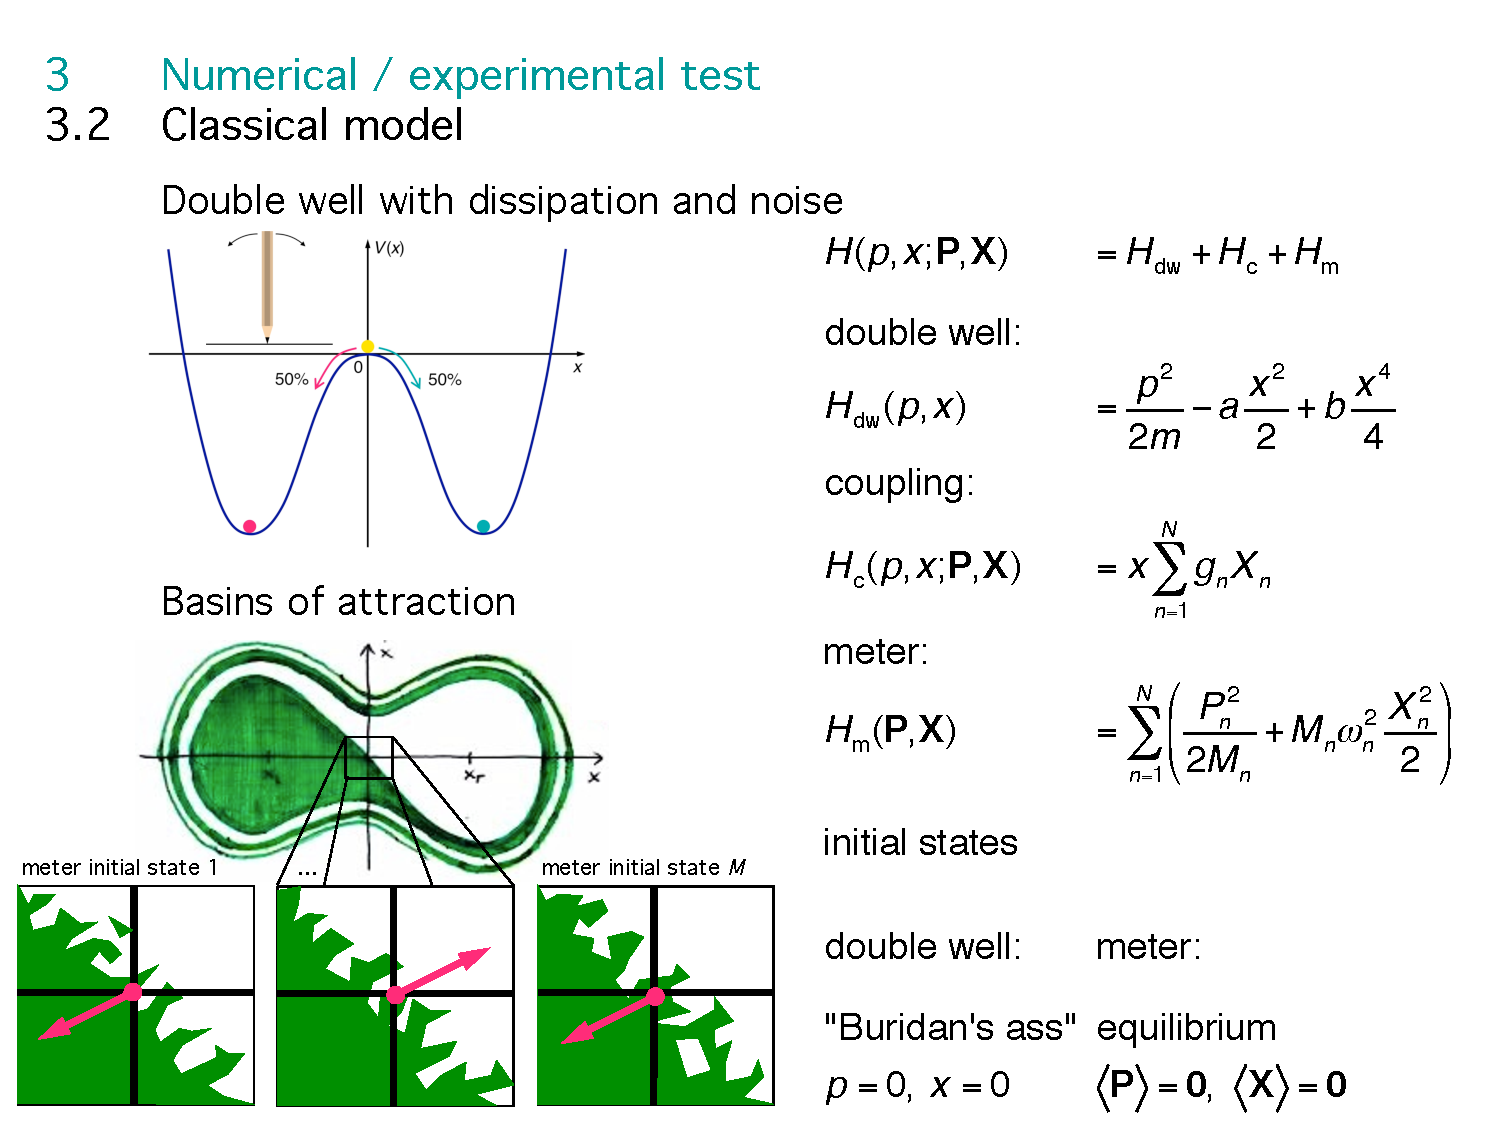
\includegraphics[width=1\linewidth]{clspinmeasmnt.pdf}
\end{center}
\caption{Hamiltonianos del sistema}
\label{fig_hamiltonianos_del_sistema}
\end{figure}

Para este sistema se tiene el siguiente hamiltoniano:
\begin{equation}
H(p,x;\textbf{P,X})=H_{dw}+H_c+H_m
\end{equation}
Con el Hamiltoniano del pozo doble (cuartico) dado por:
\begin{equation}
H_{dw}=\frac{p^2}{2m}-a\frac{x^2}{2}+b\frac{x^4}{4}
\end{equation}

El del acoplamiento dado por:
\begin{equation}
H_c(p,x;\textbf{P,X})=x\sum_{n=1}^N g_n X_n
\end{equation}
Y el del medidor:
\begin{equation}
H_m(\textbf{P,X})= \sum_{n=1}^N \Big(\frac{P_n^2}{2M_n}+M_n \omega_n^2\frac{X_n^2}{2} \Big)
\end{equation}
Las ecuaciones de Hamilton para el pozo son:
\begin{equation}
\dot{p}=\frac{-\partial H}{\partial x}=ax-bx^3-\sum_{n=1}^N g_n X_n
\end{equation}
\begin{equation}
\dot{v}=\frac{-1}{m}\frac{\partial H}{\partial x}=\frac{ax}{m}-\frac{bx^3}{m}-\frac{\sum_{n=1}^N g_n X_n}{m}
\end{equation}
\begin{equation}
\dot{x}=\frac{\partial H}{\partial p}=\frac{p}{m}
\end{equation}
Las ecuaciones de Hamilton para los osciladores son:
\begin{equation}
\dot{P_i}=\frac{-\partial H}{\partial X_i}=-xg_i-M_i \omega _i ^2 X_i
\end{equation}
\begin{equation}
\dot{V_i}=\frac{-1}{M_i}\frac{\partial H}{\partial X_i}=\frac{-xg_i}{M_i}-\omega _i^2 X_i
\end{equation}
\begin{equation}
\dot{X_i}=\frac{\partial H}{\partial P_i}=\frac{P_i}{M_i}
\end{equation}

Ahora bien, para calcular las frecuencias de pequeñas oscilaciones del pozo doble se procede de la siguiente manera. El potencial del pozo está dado por:
\begin{equation}
V(x)=-\frac{1}{2}ax^2+\frac{1}{4}bx^4
\end{equation}
Los puntos de equilibrio ocurren cuando el potencial $V$ es máximo o mínimo, es decir:
\begin{equation}
\frac{d}{dx}V=0\rightarrow x(bx^2-a) = 0
\end{equation}

Las raices de la ecuación anterior son $x=0,\pm \sqrt{\frac{a}{b}}$, donde $x=0$ es un punto de equilibrio inestable y $x=\pm \sqrt{\frac{a}{b}}$ son puntos de equilibrio estables.

Ahora bien, hacemos una expansión de Taylor alrededor del punto de equilibrio estable $x_0=\sqrt{\frac{a}{b}}$:
\begin{equation}
U(x_0 +\epsilon )=U(x_0)+U'(x_0)\epsilon + \frac{1}{2}U''(x_0)\epsilon ^2 + ...
\end{equation}
El primer término es una constante entonces se puede ignorar, el segundo término es cero ya que $U'(x_0)=0$ y el tercer término será $\frac{1}{2}(-a+3bx^2)| _{x=x_0}$, esto da como resultado:
\begin{equation}
U=\frac{1}{2}(2a)\epsilon ^2
\end{equation}
Es claro que la constante elástica de este potencial es $2a$ (por comparación con $U=\frac{1}{2}kx^2$). Esto quiere decir que la frecuencia de pequeñas oscilaciones en estos puntos de equilibrio están dadas por:
\begin{equation}
\omega =\sqrt{\frac{k}{m}}=\sqrt{\frac{2a}{m}}
\end{equation}

\experiment{Códigos para las ecuaciones de Hamilton de para 1 oscilador acoplado}
\begin{lstlisting}[language=Python]
def A(m0, a0, b0, x0, g0, X0): #p punto
    return a0*x0/m0 - b0*x0*x0*x0/m0 -(g0*X0)/m0
def V(m0,p0): #equis punto
    return p0/m0
def Ai(Mi0,wi0,x0,gi0,Xi0): #P punto sub i
    return -x0*gi0/Mi0-wi0**2.*Xi0
def Vi(Mi0,Pi0): #Equis punto sub i
    return Pi0/Mi0
\end{lstlisting}

\experiment{Código para el integrador de Ruth de 4to orden}
\begin{lstlisting}[language=Python]
def ruth4th(xx,pp,mm,XX01,PP01,MM1,ww1,gacople,dt,
iteraciones,a_poso,b_poso)#defino funcion con el integrador simplectico Ruth de 4to orden

dos=2.**(1./3.) #constante necesaria

aa=[a,(1./(2.-dos)),(-dos/(2.-dos)),(1./(2.-dos)),0] #constantes de la posicion del integrador
bb=[b,(1./(2.*(2.-dos))),(1.-dos)/(2.*(2.-dos)), (1.-dos)/(2.*(2.-dos)),(1./(2.*(2.-dos)))] #constantes de la velocidad del integrador

    x = [xx] #posicion inicial
    p = [pp] #momento inicial
    X1 = [XX01] #posicion inicial del primer oscilador
    P1 = [PP01] #momento inicial del primer oscilador
    t  = [0.] #lista de tiempo
    
    xi , pi , X1i , P1i= xx, pp , XX01 , PP01
    for i in range (iteraciones):
        vini = pi/m
        vv = V(mm,pi)+bb[1]*A(mm,a_poso,b_poso,xi,gacople,X1i)*dt
        VV1 = Vi(MM1,P1i)+bb[1]*Ai(MM1,ww1,xi,gacople[1],X1i)*dt
        xx = xi + aa[1]*vv*dt
        XX1 =XX1i + aa[1]*VV1*dt
        for j in range(2,len(aa)):
            vv += bb[j]*A(mm,a_poso,b_poso,xx,gacople,XX1)*dt
	    VV1 += bb[j]*Ai(MM1,ww1,xx,gacople[1],XX1)*dt
            xx += aa[j]*vv*dt
            XX1 += aa[j]*VV1*dt

        xi = xx
        pi = m*vv
        X1i = XX1
        P1i = MM1*VV1

        x.append(xi)
        p.append(pi) 
        X1.append(X1i)
        P1.append(P1i) 
        t.append(t[-1] + dt)
\end{lstlisting}

\experiment{Código para integrador de Yoshida de 6to orden}
\begin{lstlisting}[language=Python]
#codigo con el integrador de yoshida de sexto orden, los parametros son xx=posicion inicial, pp=momento inicial, XX01=posicion inicial del primer oscilador, PP01=momento inicial del primer oscilador, MM1=masa del primer  oscilador, ww1=frecuencia del primer oscilador, gacople= lista de los acoples para cada oscilador, dt= paso del integrador, iteraciones= numero de iteraciones del integrador, a_poso=parametro a del poso, b_poso=parametro b del poso, 

def yoshida(xx,pp,mm,XX01,PP01,MM1,ww1,gacople,dt,iteraciones,a_poso,b_poso):  #defino funcion con el integrador simplectico yoshida de 6to orden


aa = [ a, 0.78451361047756, 0.23557321335936,  -1.1776799841789,   1.3151863206839,  -1.1776799841789,  0.23557321335936, 0.78451361047756, 0]
bb = [ b, 0.39225680523878, 0.51004341191846, -0.47105338540976, 0.068753168252520, 0.068753168252520, -0.47105338540976, 0.51004341191846, 0.39225680523878]

    
    x = [xx] #posicion inicial
    p = [pp] #momento inicial
    X1 = [XX01] #posicion inicial del primer oscilador
    P1 = [PP01] #momento inicial del primer oscilador
    t  = [0.] #lista de tiempo
    
    xi , pi , X1i , P1i= xx, pp , XX01 , PP01
    for i in range (iteraciones):
        vini = pi/m
        vv = V(mm,pi)+bb[1]*A(mm,a_poso,b_poso,xi,gacople,X1i)*dt
        VV1 = Vi(MM1,P1i)+bb[1]*Ai(MM1,ww1,xi,gacople[1],X1i)*dt
        xx = xi + aa[1]*vv*dt
        XX1 =XX1i + aa[1]*VV1*dt 
        for j in range(2,len(aa)):
            vv += bb[j]*A(mm,a_poso,b_poso,xx,gacople,XX1)*dt
	    VV1 += bb[j]*Ai(MM1,ww1,xx,gacople[1],XX1)*dt
            xx += aa[j]*vv*dt
            XX1 += aa[j]*VV1*dt

        xi = xx
        pi = m*vv
        X1i = XX1
        P1i = MM1*VV1

        x.append(xi)
        p.append(pi)
        X1.append(X1i)
        P1.append(P1i) 
        t.append(t[-1] + dt)
 \end{lstlisting}   
        
\experiment{Resumen y lo que falta por hacer de hoy}
Los desarrollos anteriores fueron hechos con el fin de tener a la mano las ecuaciones útiles a las cuales vuelvo constantemente. Los códigos por otra parte, son tentativos.
Lo que debo hacer en la próxima sesión:
\begin{itemize}
\item Comprobar que los códigos propuestos funcionen, con casos de prueba
\item Agregar un código de Ruth de 3er orden
\item Una vez que los códigos funcionen, crear un código para el sistema mio que llame las funciones de los integradores
\item Cuando lo anterior sea hecho, agregar los códigos al repositorio de github
\end{itemize}
%-----------------------------------------

\experiment{example2} % Multiple experiments can be included in a single day, this allows you to segment what was done each day into separate categories

\begin{figure}[H] % Example of including images
\begin{center}

\includegraphics[width=0.5\linewidth]{example_figure}
\end{center}
\caption{Example figure.}
\label{fig:example_figure}
\end{figure}

\experiment{Rápidamente como recuperar los archivos que estaba copiando en el ssh}
\begin{lstlisting}
rsync -P -e ssh spenam@168.176.92.190:mec_estadistica/lambda09.dat /home/santiago/Downloads/mec_estadistica/proycod/09
\end{lstlisting}

%-----------------------------------------
\labday{Sábado, 16 Febrero 2019}

\experiment{Código de Ruth de 3er orden}
\begin{lstlisting}[language=Python]
def ruth3rd(xx,pp,mm,XX01,PP01,MM1,ww1,gacople,dt,
iteraciones,a_poso,b_poso)#defino funcion con el integrador simplectico Ruth de 3er orden

aa=[a,-1./24.,3./4.,7./24.] #constantes de la posicion del integrador
bb=[b,1.,-2./3., 2./3.] #constantes de la velocidad del integrador

    x = [xx] #posicion inicial
    p = [pp] #momento inicial
    X1 = [XX01] #posicion inicial del primer oscilador
    P1 = [PP01] #momento inicial del primer oscilador
    t  = [0.] #lista de tiempo
    
    xi , pi , X1i , P1i= xx, pp , XX01 , PP01
    for i in range (iteraciones):
        vini = pi/m
        vv = V(mm,pi)+bb[1]*A(mm,a_poso,b_poso,xi,gacople,X1i)*dt
        VV1 = Vi(MM1,P1i)+bb[1]*Ai(MM1,ww1,xi,gacople[1],X1i)*dt
        xx = xi + aa[1]*vv*dt
        XX1 =XX1i + aa[1]*VV1*dt
        for j in range(2,len(aa)):
            vv += bb[j]*A(mm,a_poso,b_poso,xx,gacople,XX1)*dt
	    VV1 += bb[j]*Ai(MM1,ww1,xx,gacople[1],XX1)*dt
            xx += aa[j]*vv*dt
            XX1 += aa[j]*VV1*dt

        xi = xx
        pi = m*vv
        X1i = XX1
        P1i = MM1*VV1

        x.append(xi)
        p.append(pi) 
        X1.append(X1i)
        P1.append(P1i) 
        t.append(t[-1] + dt)
\end{lstlisting}

\experiment{más dilemas con los códigos!!!!}
Hice los códigos usando los loops, para intentar hacer casos de prueba tomé el potencial caótico de Henon-Heiles, pero oh sorpresa, no obtenía la misma figura. Obtenía algo cercano pero no exactamente lo que necesitaba.\par

En un momento de desesperación, busqué alternativas. Estas posibles alternativas llegaron en Mathematica y voy a probar en Matlab(Octave). \par
Ocurre que busqué en internet posibles integradores simplécticos de Mathematica y obtengo resultados un poco distintos para los mismo parámetros a los que ya les había hecho 123081324796 gráficas! Algo bueno es que estas gráficas de Mathematica también dependen aparentemente del paso del integrador.\par
Estas imágenes muestran lo que quiero decir para los parámetros dados por: $m=0.1$, $a=0.25$, $b=0.01$, $M=0.01$, $\omega=2.236067977$,$g=0.01$ y condiciones iniciales dadas por $P(0)=0.1,X(0)=0.1$ para un tiempo t =300:\par

Todo esto usando integradores simplécticos de 4to orden.

\begin{itemize}
\item Para $dt=0.001$:


\begin{figure}[H] % Example of including images
\begin{center}
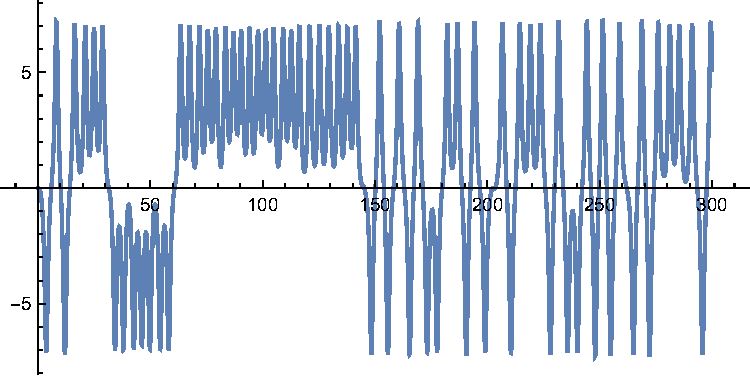
\includegraphics[width=1\linewidth]{discensopara0-001.pdf}
\end{center}
\caption{Gráfica $x$ vs $t$ en Mathematica para $dt=0.001$}
\label{graficamathematica1}
\end{figure}

\begin{figure}[H] % Example of including images
\begin{center}
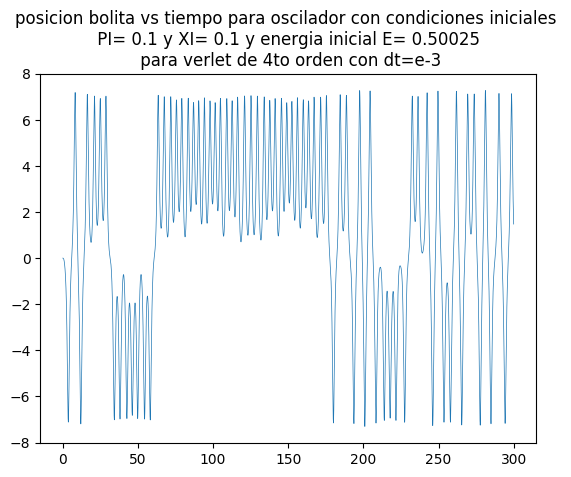
\includegraphics[width=1\linewidth]{0verlet_dt_0-001_x_vs_t_bolita.png}
\end{center}
\caption{Gráfica $x$ vs $t$ en Python para $dt=0.001$}
\label{graficapython1}
\end{figure}

\item Para $dt=0.0001$:

\begin{figure}[H] % Example of including images
\begin{center}
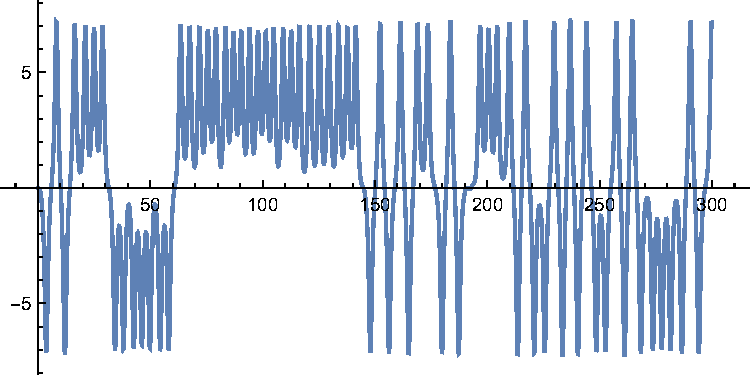
\includegraphics[width=1\linewidth]{discensopara0-0001.pdf}
\end{center}
\caption{Gráfica $x$ vs $t$ en Mathematica para $dt=0.0001$}
\label{graficamathematica2}
\end{figure}

\begin{figure}[H] % Example of including images
\begin{center}
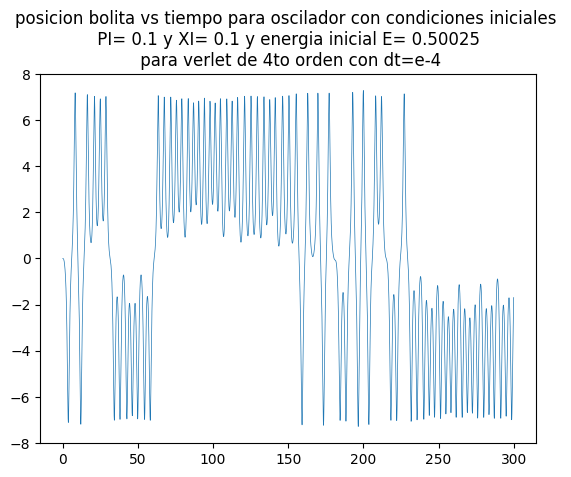
\includegraphics[width=1\linewidth]{0verlet_dt_0-0001_x_vs_t_bolita.png}
\end{center}
\caption{Gráfica $x$ vs $t$ en Python para $dt=0.0001$}
\label{graficapython1}
\end{figure}
\end{itemize}

\experiment{Resumen y lo que falta por hacer de hoy v2}
La búsqueda de los integradores simplécticos que tengan buenos resultados para este sistema empieza a ser cada vez más complicada.
Lo que debo hacer en la próxima sesión otra vez:
\begin{itemize}
\item Comprobar que los códigos propuestos funcionen, con casos de prueba
\item Una vez que los códigos funcionen, crear un código para el sistema mio que llame las funciones de los integradores
\item Cuando lo anterior sea hecho, agregar los códigos al repositorio de github
\item Hablar con Óscar y el profesor para ver que opinan al respecto.
\end{itemize}


%-----------------------------------------
\labday{Lunes, 25 Febrero 2019}
\experiment{Secciones de poincaré para m=1a=0-25b=0-01M=0-1w=0-8g=0-1 y condiciones iniciales bolita quieta y oscilador P=X=0.1}
Hice un gif usando 30 secciones de poincaré para el mismo problema, las secciones se crean a partir de tomar la frecuencia del oscilador $\omega$ aunque ahora que lo pienso, debí haber tomado el periodo del oscilador. Me pregunto si dará lo mismo.\par

Entonces esta primera parte será para la frecuencia, la otra parte será para el periodo:
\begin{itemize}
\item gif de sección de poincaré variando un poco el término de la frecuencia:


\end{itemize}
No pude agregar gifs a este archivo jajaja. Entonces me contento con haberle enviado al profesor los gifs de las secciones de poicaré para la frecuencia y periodo del oscilador.

Los otros objetivos siguen siendo los mismos:

\begin{itemize}
\item Comprobar que los códigos propuestos funcionen, con casos de prueba
\item Una vez que los códigos funcionen, crear un código para el sistema mio que llame las funciones de los integradores
\item Cuando lo anterior sea hecho, agregar los códigos al repositorio de github
\item Hablar con Óscar y el profesor para ver que opinan al respecto.
\end{itemize}

%-----------------------------------------
\labday{Domingo, 17 Marzo 2019}
\experiment{Secciones de poincaré ya que las anteriores no sirvieron}
Dado que las secciones de poincaré que intenté hacer anteriormente no funcionaron, entonces procedí a buscar bien cómo se hacían, en esto encontré un algoritmo que creo que funcionará:

Procedimiento computacional (Algoritmo para el problema de Henon-Heiles):


El procedimiento seguido en este trabajo para calcular las secciones de Poincaré en el sistema de Hénon-Heiles es el siguiente (se ha empleado el plano $x = 0$ por simplicidad, pero se podría emplear cualquier otro plano).

\begin{enumerate}
\item Se parten de unas condiciones iniciales tales que $x(0) = 0$, $y(0) = y_0$, $p_y(0) = p_{y0}$ y una energía $H = H_0$. A partir de estos valores, se calcula $p_x(0)$ a partir de la restricción $H = H_0$.
\begin{equation}
p_x(0)=\sqrt{2H_0-p_{y0}^2-y_0^2+\frac{2}{3}y_0^3}
\end{equation}
\item Se integra el sistema de ecuaciones diferenciales (4.6) con el integrador simpléctico de orden 4 empleado en todo el trabajo.

\item De la integración de las ecuaciones, el programa almacena los pares $(y,p_y)$ que cumplen que $−\epsilon < x < \epsilon$. Siendo $\epsilon$ un parámetro del programa que indica la precisión del mapa de Poincaré. Cuanto menor sea $\epsilon$, menos puntos tendrá el mapa de Poincaré resultante.

\item Una vez se han integrado las ecuaciones y se han almacenado en un archivo todos los pares $(y,p_y)$ para esta condición inicial, se vuelve al primer paso cambiando las condiciones iniciales con la misma energía y se repite todo el proceso.

\item Repitiendo este procedimiento varias veces se obtiene el mapa de Poincaré asociado al sistema dinámico (cuantas más veces repita, más rico será el mapa).

\end{enumerate}

Con esto en mente, el proceso para el hamiltoniano de nuestro problema será usando la posición del primer oscilador en $X=0$:

\begin{enumerate}
\item Se parten de unas condiciones iniciales tales que $X(0) = 0$, $p(0) = p_0$, $x(0) = x_{0}$ y una energía $H = H_0$. A partir de estos valores, se calcula $P(0)$ a partir de la restricción $H = H_0$.
\begin{equation}
P(0)=\sqrt{2M ( H_0-\frac {p_{0}^2}{2m}+a\frac {x_{0}^2}{2}-b\frac {x_{0}^4}{4})}
\end{equation}
\item Se integra el sistema de ecuaciones diferenciales (4.6) con el integrador simpléctico de orden 4 empleado en todo el trabajo.

\item De la integración de las ecuaciones, el programa almacena los pares $(y,p_y)$ que cumplen que $−\epsilon < x < \epsilon$. Siendo $\epsilon$ un parámetro del programa que indica la precisión del mapa de Poincaré. Cuanto menor sea $\epsilon$, menos puntos tendrá el mapa de Poincaré resultante.

\item Una vez se han integrado las ecuaciones y se han almacenado en un archivo todos los pares $(y,p_y)$ para esta condición inicial, se vuelve al primer paso cambiando las condiciones iniciales con la misma energía y se repite todo el proceso.

\item Repitiendo este procedimiento varias veces se obtiene el mapa de Poincaré asociado al sistema dinámico (cuantas más veces repita, más rico será el mapa).

\end{enumerate}
 
 La manera como voy a proceder es haciendo una grilla de 25 puntos al rededor de la zona de equilibrio del oscilador y manteniendo una energía fija, en la primera prueba la energía impuesta es la resultante de las condiciones iniciales del oscilador dadas por $X=0.1$ y $P=0.1$.
 




Los otros objetivos siguen siendo los mismos:
\begin{itemize}
\item Comprobar que los códigos propuestos funcionen, con casos de prueba
\item Una vez que los códigos funcionen, crear un código para el sistema mio que llame las funciones de los integradores
\item Cuando lo anterior sea hecho, agregar los códigos al repositorio de github
\item Hablar con Óscar y el profesor para ver que opinan al respecto.
\end{itemize}


%----------------------------------------
\labday{Martes, 19 Marzo 2019}
\experiment{Comandos para conectarse por ssh}
ssh spenam@168.176.92.190

la contraseña es el usuario: spenam

desde fuera del ssh copio los archivos que necesito por medio de: 
\begin{lstlisting}[language=bash]
scp route to file/file userid@168.176.92.190:Path where to save/
\end{lstlisting}
ejemplo de lo anterior: 
\begin{lstlisting}[language=bash]
scp ~/Desktop/tesis/poincare/compu_grupo/test_grupo.py spenam@168.176.92.190:poincare/
\end{lstlisting}
para traer archivos, en este caso fue una carpeta:
\begin{lstlisting}[language=bash]
scp -r chaosg@168.176.92.190:poincare  ~/Desktop/tesis/poincare/
\end{lstlisting}


Tambien puedo conectarme al cluster de Delaware por medio de este comando:
\begin{lstlisting}[language=bash]
ssh spenam@asterix-login.physics.udel.edu
\end{lstlisting}
La contrasena es la de todo.


%----------------------------------------
\labday{Sabado, 13 Abril 2019}
\experiment{Parece que el integrador funciona pero a la ves no funciona}

Definitivamente no entiendo esto de los integradores, puesto que decidí usar la base del que estaba generalizado, en donde solo tengo que insertar las constantes que definen el integrador. Decidí probar las secciones de Poincaré del potencial caotico de Henon-Heiles (El cual está más arriba) y usé un integrador de ruth de 3er orden. Luego de jugar con eso y buscar las aparentes condiciones iniciales que funcionaban, el resultado fueron gráficas bastante bonitas en donde creí que todo estaba empezando a dar:

\begin{figure}[H] % Example of including images
\begin{center}
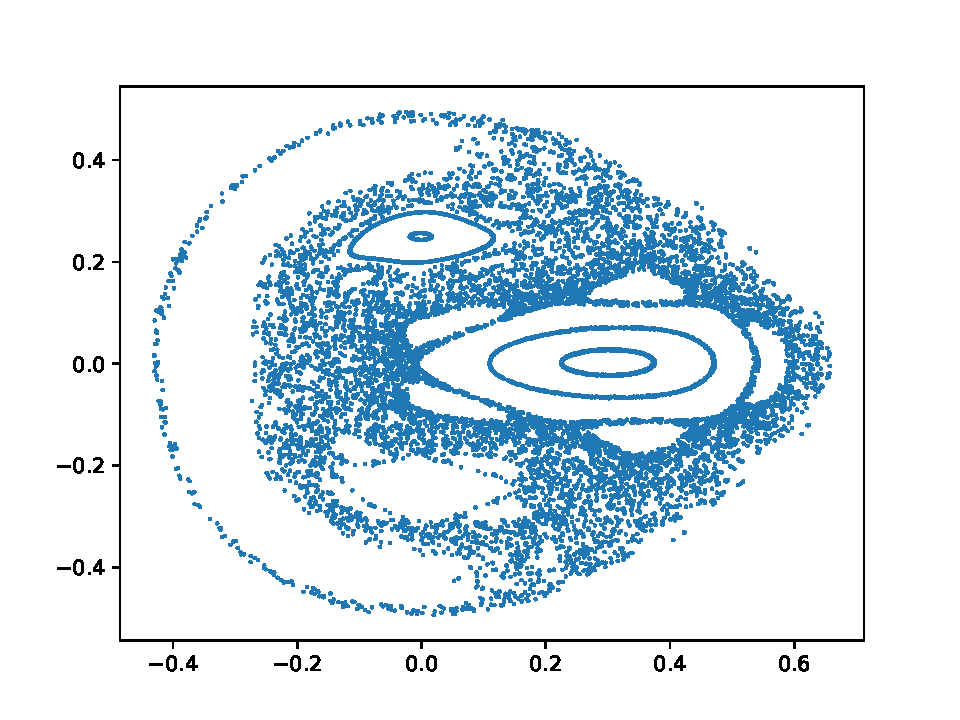
\includegraphics[width=1\linewidth]{henon_poinc.pdf}
\end{center}
\caption{Secciones de Poincaré para el potencial de Henon-Heiles}
\label{graficamathematica1}
\end{figure}

Parecía que lo había logrado, este es el código que usé:

\begin{lstlisting}[language=Python]
import math as m
import numpy as np
from matplotlib import pyplot as plt

def xpunto(vx0): #time derivative of x
    return vx0
def pxpunto(x0,y0,lambda0): #time derivative of px
    #print (x0,lambda0,y0)
    return -x0-(2.*lambda0*x0*y0)
def ypunto(vy0): #time derivative of y
    return vy0
def pypunto(x0,y0,lambda0): #time derivative of py
    return -y0-(lambda0*((x0*x0)-(y0*y0)))
def energia_poinc(y0,py0, H0): #initial condition for px using the constraints
    print (y0,py0,H0)
    print ((2.*H0)-(py0*py0)-(y0*y0)+((2./3.)*(y0*y0*y0)))
    return m.sqrt(abs((2.*H0)-(py0*py0)-(y0*y0)+((2./3.)*(y0*y0*y0))))



iteraciones=500000
dt=0.01
t=[0.]
x=[]
y=[]
px=[]
py=[]

def ruth3rd(xx,yy,ppx,ppy,lambda00):#define function with symplectic integrator

    aa=[1,-1./24.,3./4.,7./24.] #constants for position variable of the integrator
    bb=[1,1.,-2./3., 2./3.] #constants of velocity of the integrator
    
    x.append(xx)
    y.append(yy)
    px.append(ppx)
    py.append(ppy)
    

    
    xi , yi , pxi , pyi= xx, yy, ppx , ppy
    for i in range (iteraciones):
        #print (i*1.0*100.0/(iteraciones*1.0))
        vvx = pxi+bb[1]*pxpunto(xi,yi,lambda00)*dt
        VV1y = pyi+bb[1]*pypunto(xi,yi,lambda00)*dt
        xx = xi + aa[1]*vvx*dt
        yy =yi + aa[1]*VV1y*dt
        for j in range(2,len(aa)):
            vvx += bb[j]*pxpunto(xx,yy,lambda00)*dt
	    VV1y += bb[j]*pxpunto(xx,yy,lambda00)*dt
            xx += aa[j]*vvx*dt
            yy += aa[j]*VV1y*dt

        xi = xx
        pxi = vvx
        yi = yy
        pyi = VV1y

        x.append(xi)
        px.append(pxi) 
        y.append(yy)
        py.append(pyi) 
        t.append(t[-1] + dt)

setsrange=4
sets=np.array(np.linspace(0., 4., 4),dtype=np.float64)
sets1=[1.,2.,3.,4.]

for I in range(1):
    
    xpoinc=[]
    ppoinc=[]
    
    for ii in range (setsrange):
        for jj in range (setsrange):
            
            Hinicial=1./8.
            x=[0.] 
            y=[-0.15+0.3*(sets[jj]/(4.-1.))]
            py=[-0.15+0.3*(sets[ii]/(4.-1.))]
            #print(y[0],py[0],Hinicial) 
            #print(energia_poinc(y[0],py[0],Hinicial))
            px=[energia_poinc(y[0],py[0],Hinicial)] 
            
            ruth3rd(x[0],y[0],px[0],py[0],1.)       
        

	    crossings=[]
            crossingsindex=[]    
            for idx, item in enumerate(x[:-1]): #intersections
                if x[idx] < 0 and x[idx+1] > 0:
                    crossings.append(x[idx])
                    crossingsindex.append(idx)
                
            
            for index in crossingsindex:
                xpoinc.append(y[index])
                ppoinc.append(py[index])

np.savetxt('xpoinc.out',xpoinc) #data of the poincare plot
np.savetxt('ppoinc.out',ppoinc)
\end{lstlisting}

Parecía que todo iba viento en popa, pero al intentar hacer lo mismo con un integrador de cuarto orden de ruth no daba lo mismo. No daba lo mismo!!!!!! A pesar de que solo cambié las constantes, el integrador fallaba y daba valores demasiado grandes, no entiendo porqué:

\begin{lstlisting}[language=Python]
import math as m
import numpy as np
from matplotlib import pyplot as plt

def xpunto(vx0): #time derivative of x
    return vx0
def pxpunto(x0,y0,lambda0): #time derivative of px
    print (x0,lambda0,y0)
    return -x0-(2.*lambda0*x0*y0)
def ypunto(vy0): #time derivative of y
    return vy0
def pypunto(x0,y0,lambda0): #time derivative of py
    return -y0-(lambda0*((x0*x0)-(y0*y0)))
def energia_poinc(y0,py0, H0): #initial condition for px using the constraints
    print (y0,py0,H0)
    print ((2.*H0)-(py0*py0)-(y0*y0)+((2./3.)*(y0*y0*y0)))
    return m.sqrt(abs((2.*H0)-(py0*py0)-(y0*y0)+((2./3.)*(y0*y0*y0))))




iteraciones=2000
dt=0.01
t=[0.]
x=[]
y=[]
px=[]
py=[]

def ruth3rd(xx,yy,ppx,ppy,lambda00):#define function with symplectic integrator

    dos=np.math.pow(2.0, 1.0/3.0)
    aa=[1,0.5/ (2.0 - dos), 0.5*(1.0-dos)/ (2.0 - dos), 0.5*(1.0-dos)/ (2.0 - dos), 0.5/ (2.0 - dos)] #constants for position variable of the integrator
    bb=[1,1./ (2.0 - dos),-dos/ (2.0 - dos),1./ (2.0 - dos),0.] #constants of velocity of the integrator
    
    x.append(xx)
    y.append(yy)
    px.append(ppx)
    py.append(ppy)
    

    
    xi , yi , pxi , pyi= xx, yy, ppx , ppy
    for i in range (iteraciones):
        #print (i*1.0*100.0/(iteraciones*1.0))
        vvx = pxi+bb[1]*pxpunto(xi,yi,lambda00)*dt
        VV1y = pyi+bb[1]*pypunto(xi,yi,lambda00)*dt
        xx = xi + aa[1]*vvx*dt
        yy =yi + aa[1]*VV1y*dt
        for j in range(2,len(aa)):
            vvx += bb[j]*pxpunto(xx,yy,lambda00)*dt
	    VV1y += bb[j]*pxpunto(xx,yy,lambda00)*dt
            xx += aa[j]*vvx*dt
            yy += aa[j]*VV1y*dt

        xi = xx
        pxi = vvx
        yi = yy
        pyi = VV1y

        x.append(xi)
        px.append(pxi) 
        y.append(yy)
        py.append(pyi) 
        t.append(t[-1] + dt)

setsrange=2
sets=np.array(np.linspace(0., 4., 4),dtype=np.float64)
sets1=[1.,2.,3.,4.]

for I in range(1):
    
    xpoinc=[]
    ppoinc=[]
    
    for ii in range (setsrange):
        for jj in range (setsrange):
            
            Hinicial=1./8.
            x=[0.] 
            y=[-0.15+0.3*(sets[jj]/(4.-1.))]
            py=[-0.15+0.3*(sets[ii]/(4.-1.))]
            #print(y[0],py[0],Hinicial) 
            #print(energia_poinc(y[0],py[0],Hinicial))
            px=[energia_poinc(y[0],py[0],Hinicial)] 
            
            ruth3rd(x[0],y[0],px[0],py[0],1.)       
        

	    crossings=[]
            crossingsindex=[]    
            for idx, item in enumerate(x[:-1]): #intersections
                if x[idx] < 0 and x[idx+1] > 0:
                    crossings.append(x[idx])
                    crossingsindex.append(idx)
                
            
            for index in crossingsindex:
                xpoinc.append(y[index])
                ppoinc.append(py[index])

np.savetxt('xpoinc4th.out',xpoinc) #data of the poincare plot
np.savetxt('ppoinc4th.out',ppoinc)
\end{lstlisting}

Hice también varias pruebas numéricas de los integradores para el caso del péndulo y muestra que conserva bien el area, entonces no se que está pasando.\par

Por fin encontré el error, estaba en el algoritmo del integrador, estaba llamando pxpunto en el paso de evolución de VV1y!!!!!!!!!!!!!!!!!!!!!!!!!!!!!!!!!!!!!!!!!!!!!!!!!!!



%----------------------------------------
\labday{Viernes, 19 Abril 2019}
\experiment{Algoritmo terminado para los integradores}

Luego de que por fin tuviera bien aparentemente los integradores los probé con el sistema y obtuve unos resultados aparentemente satisfactorios, en la carpeta de poincare que se llama pruba integrador hice los codigos llamados 3rdsistema y 4th sistema donde supuestamente los tengo en el modo del algoritmo y aparentemente funciona bastante bien. Ahora voy a estudiar los papers que me mandó Thomas donde implementan unos métodos de integradores simplecticos sin constantes negativas donde argumentan que las constantes negativas dan inestabilidad en la integracion. Algo interesante es que probé esto con el caso que tiene una frecuencia bastante alta y la grafica no coincidio con ninguna que habia hecho anteriormente lo cual me genera bastante curiosidad.


%----------------------------------------
\labday{Lunes, 29 Abril 2019}
\experiment{Papers de nuevos integradores simplecticos que thomas me paso}

En los papers que thomas me mando usan unos integradores simplecticos de segundo orden llamados $SABA_2$ y $SBAB_2$, estos algoritmos pueden ser generalizados para cualquier orden en Hamiltonianos de la forma:
\begin{equation}
H=A+\epsilon B
\end{equation} 
Dadas las ecuaciones de Hamilton definidas por:
\begin{equation}
\frac{dp_n}{dt} =-\frac{\partial H}{\partial q_n},\; \frac{dq_n}{dt}=\frac{\partial H}{\partial p_n},\; n=1,2,....N
\end{equation}
Tambien recordamos los corchetes de poisson para funciones $f(p,q)$ y $g(p,q)$ los cuales son dados por:
\begin{equation}
\{ f,g \} =\sum_{n=1}^n \bigg( \frac{\partial f}{\partial p_n}\frac{\partial g}{\partial q_n}-\frac{\partial f}{\partial q_n}\frac{\partial g}{\partial p_n}\bigg)
\end{equation}
Entonces las ecuaciones de Hamilton toman la forma de:

\begin{equation}
\frac{dx}{dt}=\{H,x\}=L_H x
\end{equation}

Donde $L_H$ es el operador diferencial definido por $L_\chi f=\{ \chi ,f\}$. La solucion a la ecuacion anterior para condiciones iniciales $x(0)=x_0$ esta dada por:
\begin{equation}
x(t)=\sum_{n\geq 0}\frac{t^n}{n!}L_H^n x_0=e^{tL_H}x_0
\end{equation}
Entonces los integradores quedarían:
\begin{equation}
SABA_2=e^{c_1\tau L_A}e^{d_1\tau L_{\epsilon B}}e^{c_2\tau L_A}e^{d_1\tau L_{\epsilon B}}e^{c_1\tau L_A}
\end{equation}
con $c_1=\frac{1}{2}(1-\frac{1}{\sqrt{3}})$, $c_2=\frac{1}{\sqrt{3}}$ y $d_2=\frac{1}{2}$, mientras que el otro integrador queda:
\begin{equation}
SBAB_2=e^{d_1\tau L_{\epsilon B}}e^{c_2\tau L_A}e^{d_2\tau L_{\epsilon B}}e^{c_2\tau L_A}e^{d_1\tau L_{\epsilon B}}
\end{equation}
con $c_2=\frac{1}{2}$, $d_1=\frac{1}{6}$ y $d_2=\frac{2}{3}$. Al usar estos integradores estamos aproximando el comportamiento dinamico del Hamiltoniano real $H=A+\epsilon B$ por el Hamiltoniano $\widetilde{H} = A+\epsilon B + \mathcal{O} (\tau ^4\epsilon +\tau ^2 \epsilon ^2)$.\par 
La precision de los integradores puede ser mejorada al introducir el termino $C=\{\{A,B\},B\}$ lo cual lleva a un sistema integrable. Esto agrega unos pequenos pasos que pueden ser agregados al integrador:

\begin{equation}
SABA_2C=e^{-(\tau^3\epsilon^2g/2)L_C}(SABA_2)e^{-(\tau^3\epsilon^2g/2)L_C}
\end{equation}
Una expresion similar puede ser derivada para  $SBAB_2$ donde el valor de $g$ se escoge de tal manera que elimine la dependencia de $\tau^2\epsilon^2}$ asi el integrador queda con el orden de $\mathcal{O}(\tau^4\epsilon+\tau^4\epsilon^2$. En particular tenemos que $g=(2-\sqrt{3})/24$ para $SABA_2$ y $g=1/72$ para $SBAB_2$. Se enfatiza que estos integradores solo involucran pasos hacia adelante lo cual incrementa la estabilidad numerica.\par 

Para nuestro sistema es necesario entonces calcular los corchetes de poisson de estos casos, esto tiene como resultado:

\begin{equation}
A=\frac{p^2}{2m}+\sum_{n=1}^N \frac{P_n^2}{2M_n}
\end{equation}
\begin{equation}
B=-a\frac{x^2}{2}+b\frac{x^4}{4}+\sum_{n=1}^N M_n\omega_n^2\frac{X_n^2}{2}+x\sum_{n=1}^N g_nX_n
\end{equation}
\begin{equation}
L_Ax=\frac{p}{m}
\end{equation}
\begin{equation}
L_AX_n= \frac{P_n}{M_n}
\end{equation}
\begin{equation}
L_Ap=L_AP=0
\end{equation}
\begin{equation}
L_Bx=L_BX=0
\end{equation}
\begin{equation}
L_Bp=ax-bx^3-\sum_{n=1}^N g_nX_n
\end{equation}
\begin{equation}
L_BP_n=-M_n\omega_n^2X_n - xg_n
\end{equation}

Con esto, obtengo que:
\begin{equation}
\{\{A,B\},B\}=\frac{\big(-ax+bx^3+\sum_{n=1}^Ng_nX_n\big)^2}{m}+\sum_{n=1}^N\frac{(xg_n+M_n\omega^2_nX_n)^2}{M_n}
\end{equation}

Por lo tanto:
\begin{equation}
\begin{array}{•}
L_Cp=\frac{-2}{m}(-ax+bx^3+\sum_{n=1}^N g_nX_n)(-a+3bx^2)-\sum_{n=1}^N\frac{2}{M_n}(xg_n+M_n\omega_n^2X_n)(g_n)=\\ =\frac{-2}{m}(a^2x-abx^3-a\sum_{n=1}^N g_nX_n-3abx^3+3b^2x^5+3bx^2\sum_{n=1}^N g_nX_n)-\sum_{n=1}^N\frac{2}{M_n}(xg_n^2+M_ng_n\omega_n^2X_n)

\end{array}

\end{equation}
\begin{equation}
\begin{array}{•}
L_CP=\frac{-2}{m}(-ax+bx^3+\sum_{n'=1}^Ng_{n'}X_{n'})(g_n)-2(xg_n+M_n\omega_n^2X_n)\omega_n^2=\\
 =\frac{-2}{m}(-axg_n+bx^3g_n+\sum_{n'=1}^Ng_{n'}X_{n'}g_n)-2xg_n\omega_n^2-2M_n\omega_n^4X_n

\end{array}
\end{equation}

Entonces tengo como resultado las evoluciones de la manera siguiente:
\begin{equation}
e^{\tau L_A}:\begin{cases}
	x'=\frac{p}{m}\tau+x \\
	p'=p \\
	X_n'=\frac{P_n}{M_n}\tau+X_n \\
	P_n'=P_n \\
	\end{cases}
\end{equation}
\begin{equation}
e^{\tau L_B}:\begin{cases}
	x'=x \\
	p'=(ax-bx^3-\sum_{n=1}^Ng_nX_n)\tau+p \\
	X_n'=X_n \\
	P_n'=(-M_n\omega_n^2X_n-xg_n)\tau+P_n \\
	\end{cases}
\end{equation}

\begin{equation}
e^{-\tau L_C}:\begin{cases}
	x'=x \\
	p'=\big(\frac{-2}{m}(a^2x-abx^3-a\sum_{n=1}^N g_nX_n-3abx^3+3b^2x^5+3bx^2\sum_{n=1}^N g_nX_n) \\ -\sum_{n=1}^N\frac{2}{M_n}(xg_n^2+M_ng_n\omega_n^2X_n)\big)\tau+p \\
	X_n'=X_n \\
	P_n'=\big(\frac{-2}{m}(-axg_n+bx^3g_n+\sum_{n'=1}^Ng_{n'}g_nX_n)-(2xg_n\omega_n^2+2M_n\omega_n^4X_n)\big)\tau+P_n \\
	\end{cases}
\end{equation}

%----------------------------------------

\experiment{example3}

\lipsum[3-5]

%----------------------------------------------------------------------------------------

\labday{Friday, 26 March 2010}

\experiment{table}

\begin{table}[H]
\begin{tabular}{l l l}
\toprule
\textbf{Groups} & \textbf{Treatment X} & \textbf{Treatment Y} \\
\toprule
1 & 0.2 & 0.8\\
2 & 0.17 & 0.7\\
3 & 0.24 & 0.75\\
4 & 0.68 & 0.3\\
\bottomrule
\end{tabular}
\caption{The effects of treatments X and Y on the four groups studied.}
\label{tab:treatments_xy}
\end{table}

Table \ref{tab:treatments_xy} shows that groups 1-3 reacted similarly to the two treatments but group 4 showed a reversed reaction.

%----------------------------------------------------------------------------------------

\labday{Saturday, 27 March 2010}

\experiment{Bulleted list example} % You don't need to make a \newexperiment if you only plan on referencing it once

This is a bulleted list:

\begin{itemize}
\item Item 1
\item Item 2
\item \ldots and so on
\end{itemize}

%-----------------------------------------

\experiment{example}

\lipsum[6]

%-----------------------------------------

\experiment{example2}

\lipsum[7]

%----------------------------------------------------------------------------------------
%	FORMULAE AND MEDIA RECIPES
%----------------------------------------------------------------------------------------

\labday{} % We don't want a date here so we make the labday blank

\begin{center}
\HRule \\[0.4cm]
{\huge \textbf{Formulae and Media Recipes}}\\[0.4cm] % Heading
\HRule \\[1.5cm]
\end{center}

%----------------------------------------------------------------------------------------
%	MEDIA RECIPES
%----------------------------------------------------------------------------------------

\newpage

\huge \textbf{Media} \\ \\

\normalsize \textbf{Media 1}\\
\begin{table}[H]
\begin{tabular}{l l l}
\toprule
\textbf{Compound} & \textbf{1L} & \textbf{0.5L}\\
\toprule
Compound 1 & 10g & 5g\\
Compound 2 & 20g & 10g\\
\bottomrule
\end{tabular}
\caption{Ingredients in Media 1.}
\label{tab:med1}
\end{table}

%-----------------------------------------

%\textbf{Media 2}\\ \\

%Description

%----------------------------------------------------------------------------------------
%	FORMULAE
%----------------------------------------------------------------------------------------

\newpage

\huge \textbf{Formulae} \\ \\

\normalsize \textbf{Formula 1 - Pythagorean theorem}\\ \\
$a^2 + b^2 = c^2$\\ \\

%-----------------------------------------

%\textbf{Formula X - Description}\\ \\

%Formula

%----------------------------------------------------------------------------------------

\end{document}